
\chapter{JTWPA theory}
\label{c:twpa_theory}

The theoretical treatment of the Josephson traveling-wave parametric amplifier (JTWPA) has gone through several iterations, starting with relatively back-of-the-envelope calculations and evolving into a very complete description of the full nonlinear behavior of the device, including multiple non-idealities corresponding to the reality of the physical implementation.  I will begin this chapter with a discussion of the basic problem of phase matching in nonlinear optical devices as well as the general theory of four-wave mixing.  Next, I will lay out a rigorous theory of the JTWPA, and then describe our solution to the phase matching problem and exactly solve the dispersion relation using a standard technique from microwave network analysis.  Finally, I will present theoretical predictions for the amplifier gain, bandwidth, and input compression power.

\section{Nonlinear refraction, phase modulation, and four-wave mixing}

The language of circuit theory is appropriate to describe the behavior of lumped-element microwave networks, including lumped nonlinearities such as transistors and Josephson junctions.  Distributed networks generally consist of series of linear waveguides and lumped element components.  The literature of microwave networks in general does not treat the case of propagation in nonlinear waveguides; this is largely because high-quality, highly nonlinear, lumped-element components are commonplace in microwave electronics and are relatively straightforward to model.  At optical frequencies, however, the wavelength is so small that virtually every component in the system must be treated in the distributed limit, and thus a rich theory of continuum nonlinear wave propagation has been developed to model nonlinear optical systems.  The junction-loaded transmission line which comprises the JTWPA can be considered in this regime, as the lumped elements are in the deep-subwavelength limit and the transmission line is well approximated as a continuum.  Thus, it is natural to introduce the language of continuum nonlinear optics, and apply this existing rich theory to understand the behavior of the JTWPA.  In this section I will briefly introduce a few of the fundamental physical effects present in nonlinear optical systems, following chapters 1 and 10 of reference \cite{Agrawal2012}.  This section will be expressed in the language of single spatial mode optics, which is essentially analogous to the microwave case except for the additional polarization degree of freedom present in the optical case.

For a purely linear dielectric medium, we can write the polarization vector $\vec{P}$ of the material as
\begin{equation}
\vec{P} = \epsilon_0 \boldsymbol{\chi} \cdot \vec{E}
\end{equation}
where $\boldsymbol{\chi}$ is the material susceptibility.  In general, the polarization response of any material will become nonlinear if $|\vec{E}|$ is made large enough.  In that case, we can express the material polarization vector as a series expansion in increasing orders of $\vec{E}$
\begin{equation}
\vec{P} = \epsilon_0 \left( \boldsymbol{\chi}^{(1)} \cdot \vec{E} + \boldsymbol{\chi}^{(2)} : \vec{E}\vec{E} + \boldsymbol{\chi}^{(3)}\mathbin{\vdots} \mathbf{EEE}+ \cdots \right)
\label{eq:P_NL}
\end{equation}
where $\boldsymbol{\chi}^{(j)}$ is the $j$th order susceptibility (a rank $j+1$ tensor) and the vertical dots indicate tensor multiplication.  The second order susceptibility $\boldsymbol{\chi}^{(2)}$ vanishes for a material with spatial inversion symmetry, which will hold for our nonlinear junction-loaded transmission line.  Thus, $\boldsymbol{\chi}^{(3)}$ is the first nonlinear order to contribute, and it is this term that brings about virtually all nonlinear effects of interest, including the four-wave mixing process used in parametric amplification.

Though $\boldsymbol{\chi}^{(3)}$ is a rank-four tensor, we are only interested in one component of that tensor, the nonlinear index of refraction
\begin{equation}
n_2 = \frac{3}{8n} \textrm{Re}(\chi^{(3)}_{xxxx}).
\end{equation}
This term involves no mixing between polarization states of the electric field.  Since our microwave system lacks a polarization degree of freedom anyway, we can lump all of the effect of the $\boldsymbol{\chi}^{(3)}$ nonlinearity into this one number.  This allows us to write a simple form for the nonlinear index of refraction as
\begin{equation}
\tilde{n}(|E|^2) = n + n_2 |E|^2
\end{equation}
where $|E|^2$ is the optical intensity.  The phase of a wave that propagates through this medium for a length $L$ evolves as
\begin{equation}
\phi = \tilde{n} k_0 L = (n + n_2 |E|^2)k_0 L
\end{equation}
where $k_0 = 2\pi/\lambda$.  We can re-express this equation as the sum of two terms
\begin{equation}
\phi = \varphi_{0} + \phi_{\textrm{NL}} = n k_0 L + n_2 k_0 L |E|^2;
\end{equation}
the first term is the familiar linear phase shift, while the second term is known as \textit{self-phase modulation} (SPM) as the wave generates in itself an extra intensity-dependent phase shift.

What about a case where we have more than one wave co-propagating in this nonlinear medium?  Assuming the two waves have the same polarization, the total electric field can be written as
\begin{equation}
E = \frac{1}{2} ( E_1 e^{-i \omega_1 t} + E_2 e^{-i \omega_2 t} + \textrm{c.c.}).
\end{equation}
We plug this equation into the expression for $\phi_{\textrm{NL}}$ and neglect terms rotating at any frequency besides $\omega_1$ and $\omega_2$; the resulting nonlinear phase shift for the wave at $\omega_1$ is
\begin{equation}
\phi_{\textrm{NL}} = n_2 k_0 L ( |E_1|^2 + 2 |E_2|^2).
\end{equation}
We identify the first term as the same SPM effect we found for single-wave propagation.  The second term is now a phase shift induced in the wave at $\omega_1$ by the wave at $\omega_2$ and known as \textit{cross-phase modulation} (XPM).  Compensating these nonlinear phase shifts will be the primary challenge in realizing efficient four-wave mixing in a traveling-wave amplifier.

The physical origin of four-wave mixing is the nonlinear dependence on the electric field in the $\boldsymbol{\chi}^{(3)}$ term of (\ref{eq:P_NL}).    For four waves of the same polarization oscillating at $\omega_j$ where $j \in \{1,2,3,4\}$, we can write the total electric field as
\begin{equation}
E = \frac{1}{2} \sum^4_{j=1} E_j \exp{[i (k_j z - \omega_j t)]} +  \textrm{c.c.}
\label{eq:E_series}
\end{equation}
where the propagation constant $k_j = \tilde{n}_j \omega_j / c$ and $\tilde{n}_j$ is the nonlinear index of refraction for mode $j$.  Substituting this form into (\ref{eq:P_NL}), we find a large number of terms involving the product of three electric fields.  If we express the result as a series in the same form as (\ref{eq:E_series}), we can for instance express the total material polarization oscillating at $\omega_4$ as
\begin{align}
P_4 &= \frac{3 \epsilon_0}{4} \chi^{(3)}_{xxxx} [ |E_4|^2 E_4 + 2 (|E_1|^2 + |E_2|^2 + |E_3|^2)E_4 \notag \\
&+2E_1 E_2 E_3 \exp{(i \Theta_+)} + 2 E_1 E_2 E_3^* \exp{(i \Theta_-)} + \hdots]
\label{eq:fwm_prods}
\end{align}
where $\Theta_+$ and $\Theta_-$ are defined as
\begin{align}
\Theta_+ &= (k_1 + k_2 + k_3 - k_4)z - (\omega_1 + \omega_2 + \omega_3 - \omega_4)t,
\\ \Theta_- &= (k_1 + k_2 - k_3 - k_4)z - (\omega_1 + \omega_2 - \omega_3 - \omega_4)t.
\end{align}

We can immediately identify the term proportional to $|E_4|^2 E_4$ as SPM, and the term following it as XPM.  The remaining two terms are proportional to sum and difference frequency combinations of the waves.  When $\Theta_{\pm}$ have a nonzero value, the latter terms in \eqref{eq:fwm_prods} are oscillatory and cannot build up a large effect over the length of the device; however, when $\Theta$ is close to zero, they can contribute at the same order as the SPM and XPM terms.  In this regime these frequency-mixing terms can contribute a large effect to the total nonlinear propagation and create significant exchanges of energy in length, realizing an efficient multi-wave mixing process.

The term containing $\Theta_+$ expresses energy conservation of the form
\begin{equation}
\omega_4 = \omega_1 + \omega_2 + \omega_3
\end{equation}
where three photons combine to produce one photon.  This process is responsible for effects such as third-harmonic generation when $\omega_1 = \omega_2 = \omega_3$.  The term containing $\Theta_-$, on the other hand, destroys two photons while creating two photons, such that
\begin{equation}
\omega_3 + \omega_4 = \omega_1 + \omega_2.
\end{equation}
We are primarily interested in the case of degenerate four-wave mixing, where $\omega_1 = \omega_2$.  For this process to not be oscillatory in space, we require the satisfaction of the condition $\Delta k = 0$ where
\begin{equation}
\Delta k = k_3 + k_4 - k_1 - k_2.
\end{equation}
The propagation constants $k_j$ are themselves dependent on frequency through the dispersion relation $k(\omega)$ and also to the total field intensity through $\tilde{n}_j$.







\section{Derivation of the continuum wave equation for the JTWPA}\label{s:twpa_wave_eq}

In order to link to the continuum nonlinear optical theory developed in the last section, we need to find a continuum description of the lumped-element nonlinear transmission line forming the heart of the JTWPA.  The original derivation of the continuum nonlinear wave equation for the JTWPA was performed by Friedland and Yaakobi in our publication in Physical Review Letters \cite{Yaakobi:2013kx}.  The circuit model for a unit cell of the junction-loaded transmission line is shown in Figure \ref{fig:TWPA_circuit_model}. The basic idea is to apply Kirchoff's laws to one unit cell and its neighbors, use the translational symmetry of the transmission line to create a discrete wave equation, and then find the continuum approximation by converting finite difference relations to derivatives.

\begin{figure*}
\begin{center}
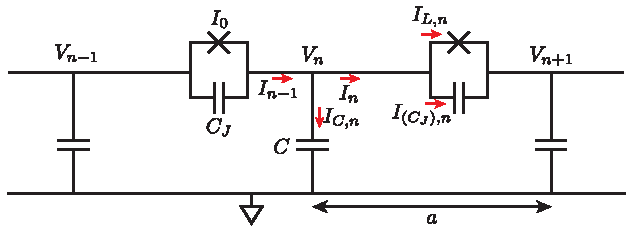
\includegraphics[width=4.2in]{twpa_theory/TWPA_circuit_model}
\end{center}
\caption[Circuit model for junction-loaded transmission line]{Circuit model for junction-loaded transmission line.  The bottom wire is connected to ground, and the conventions for voltage drop and current flow are indicated.}
\label{fig:TWPA_circuit_model}
\end{figure*}


Current conservation at each node implies
\begin{equation}
I_{n}=I_{ (C_{J}), n}+I_{L,n}.  \label{Current conservation secondary}
\end{equation}
The current in capacitor $C_{J}, n$ is related to the voltages $V_{n}$ and $V_{n+1}$\ by the derivative 
\begin{equation}
I_{ (C_{J}), n}=-C_{J}\frac{d}{dt}\left( V_{n+1}-V_{n}\right).
\label{Current voltage cj}
\end{equation}
We define the magnetic flux as the time integral of the voltage across the inductor, expressed here as a difference equation 
\begin{equation}
V_{n+1}-V_{n}=-\frac{d\Phi _{n}}{dt},
\label{Magnetic flux definition}
\end{equation}
and we write the expression for the junction current-phase relation 
\begin{equation}
I_{L,n}=I_{0}\sin \left[ \frac{\Phi _{n}}{\varphi_{0}}\right] ,
\label{Josephson current}
\end{equation}
where $\varphi_{0} = \Phi _{0}/2\pi$ is the reduced flux quantum.  Differentiation of the last equation yields
\begin{equation}
\frac{dI_{L,n}}{dt}=\frac{I_{0}}{\varphi_{0}}\left( \cos \left[ \frac{\Phi _{n}}{\varphi_{0}}\right] \right) \frac{d\Phi _{n}}{dt}.
\end{equation}
Then
\begin{equation}
\frac{d\Phi _{n}}{dt}=\frac{dI_{L,n}}{dt}\frac{\varphi_{0}}{I_{0}}\left( 1-\sin ^{2}\left[ \frac{\Phi _{n}}{\varphi_{0}}\right] \right)^{-\frac{1}{2}},
\end{equation}
which, upon using Eq. (\ref{Josephson current}), becomes
\begin{equation}
\frac{d\Phi _{n}}{dt}=\frac{\varphi_{0}}{I_{0}}\left( 1-\left[ \frac{I_{L,n}}{I_{0}}\right] ^{2}\right) ^{-\frac{1}{2}}\frac{dI_{L,n}}{dt}.
\label{Nonlinear inductance}
\end{equation}
For the weakly nonlinear regime $I_{L,n}/I_{0} \ll 1$, we approximate the nonlinear contribution to first order as
\begin{equation}
\frac{d\Phi _{n}}{dt}=\frac{\varphi_{0}}{I_{0}}\left( 1+\frac{1}{2} \left[ \frac{I_{L,n}}{I_{0}}\right] ^{2}\right) \frac{dI_{L,n}}{dt}.
\label{Weak nonlinear inductance}
\end{equation}
Since the current through capacitor $C_n$ is
\begin{equation}
I_{C,n}=-C \frac{d}{dt}\left( 0-V_{n}\right)=C\frac{dV_{n}}{dt},
\label{Capacitor current}
\end{equation}
current conservation yields
\begin{equation}
I_{n}-I_{n-1}=-C\frac{dV_{n}}{dt}.
\label{Current voltage primary}
\end{equation}
Next, we use equations 
(\ref{Magnetic flux definition}) and (\ref{Weak nonlinear inductance}) to get
\begin{equation}
V_{n+1}-V_{n}=-L\frac{dI_{L,n}}{dt}-\frac{\varphi_{0}}{6I_{0}^{3}}\frac{d}{dt}\left( I_{L,n}\right) ^{3},  \label{B}
\end{equation}
where $L=\varphi_{0}/I_{0}.$ Introducing the node fluxes $\phi_{n}$ as
\begin{equation}
V_{n}\equiv \frac{d\phi_{n}}{dt}
\label{node flux definition}
\end{equation}
and integrating (\ref{B}), we obtain
\begin{equation}
\phi_{n+1}-\phi_{n}=-LI_{L,n}-\frac{L}{6I_{0}^{2}}I_{L,n}^{3}
\label{V_n difference}
\end{equation}
where we have set the integration constant to zero. Rearranging the last equation yields
\begin{equation}
I_{L,n}=-\frac{1}{L}\left( \phi_{n+1}-\phi_{n}\right) -\frac{1}{6I_{0}^{2}}I_{L,n}^{3}.
\end{equation}
Assuming that the nonlinear term is small, we can approximate this to lowest (linear) order 
\begin{equation}
I_{L,n}\approx -\frac{1}{L}\left( \phi_{n+1}-\phi_{n}\right) .
\end{equation}
Then, by plugging this expression back into \eqref{V_n difference}, we get the first-order nonlinear approximation
\begin{equation}
I_{L,n}=-\frac{1}{L}\left( \phi_{n+1}-\phi_{n}\right) + \frac{1}{6I_{0}^{2}L^{3}}\left( \phi_{n+1}-\phi_{n}\right) ^{3}.  \label{I_Ln second iteration}
\end{equation}
Finally, combining equations (\ref{Current conservation secondary}), (\ref{Current voltage cj}), (\ref{Current voltage primary}), (\ref{node flux definition}) and (\ref{I_Ln second iteration}), we obtain the first-order nonlinear system
\begin{align}
-C \frac{d^{2}\phi_{n}}{dt^{2}} = &-C_{J}\frac{d^{2}}{dt^{2}}\left[ \phi_{n+1}+\phi_{n-1}-2 \phi_{n}\right]  \notag \\
&-\frac{1}{L}\left[ \phi_{n+1}+\phi_{n-1}-2 \phi_{n}\right]  \notag \\
&+\frac{1}{6I_{0}^{2}L^{3}}\left[ \left( \phi_{n+1}-\phi_{n}\right) ^{3}-\left( \phi_{n}-\phi_{n-1}\right) ^{3}\right].
\label{Discrete wave equation uniform}
\end{align}

At this point we could numerically solve this equation for an arbitrary number of unit cells, but this does not provide any further intuition.  We would like to make a link to the existing theory of continuum nonlinear optics; if we assume that the wavelength of a propagating mode is much larger than one unit cell ($a/\lambda \ll 1$), we can replace the discrete $n$ by a continuous position $x$ and replace the finite differences in the discrete equations by their continuous counterparts to second order in $(a/\lambda)$: 
\begin{align}
\phi_{n+1}-\phi_{n} &\approx a\frac{\partial \phi}{\partial x}+\frac{1}{2}a^{2}\frac{\partial ^{2} \phi}{\partial x^{2}} \\
\phi_{n}-\phi_{n-1} &\approx a\frac{\partial \phi}{\partial x}-\frac{1}{2}a^{2}\frac{\partial ^{2}\phi}{\partial x^{2}}
\end{align}
\begin{equation}
\phi_{n+1}+\phi_{n-1} -2\phi_{n} \approx a^{2}\frac{\partial ^{2}\phi}{\partial x^{2}}.
\end{equation}
Then, to lowest significant order in $a/\lambda$,
\begin{equation}
\left( \phi_{n+1}-\phi_{n}\right) ^{3}-\left( \phi_{n}-\phi_{n-1}\right) ^{3}\approx 3a^{4}\left( \frac{\partial ^{2}\phi}{\partial x^{2}}\right) \left( \frac{\partial \phi}{\partial x}\right) ^{2},
\end{equation}
and we arrive at the continuous counterpart of (\ref{Discrete wave equation uniform}):
\begin{equation}
C\frac{\partial ^{2}\phi}{\partial t^{2}}-\frac{a^{2}}{L} \frac{\partial ^{2}\phi}{\partial x^{2}}-C_{J}a^{2}\frac{\partial ^{4}\phi}{\partial t^{2}\partial x^{2}}+\frac{a^{4}}{2I_{0}^{2}L^{3}}\left( \frac{\partial^{2}\phi}{\partial x^{2}}\right) \left( \frac{\partial \phi}{\partial x}\right)^{2}=0.
\end{equation}
The first three terms in this expression describe weakly dispersive linear waves, while the fourth term represents the nonlinearity due to the junctions.

\section{Efficient parametric amplification}

With the continuum wave equation for the JTWPA in hand, we can attempt to find an approximate analytical solution for the behavior of several coupled waves.  This derivation is analogous to the technique used in nonlinear optics, described in chapter 10 of reference \cite{Agrawal2012}; the only major differences for this system are the presence of the weakly dispersive term due to the junction self-capacitance, and the simplicity of a purely one-dimensional problem.  This calculation was performed by Kevin O'Brien and appears as Appendix 1 in our publication in Physical Review Letters \cite{OBrien2014}.  I reproduce the full details of this calculation in Appendix \ref{a:twpa_paramp}.

By making the ansatz that the solutions are traveling waves, taking the slowly varying envelope approximation, and neglecting pump depletion (that is, assuming the energy of the pump wave remains constant over the length of the transmission line), we obtain a set of coupled wave equations which describe the energy exchange between the pump, signal, and idler:
\begin{align}
\frac{{\partial {a_s}}}{{\partial x}} - i{\kappa _s}a_i^*{e^{i(\Delta {k_L} + 2{\alpha _p} - {\alpha _s} - {\alpha _i})x}} &= 0 \label{eq:1} \\
\frac{{\partial {a_i}}}{{\partial x}} - i{\kappa _i}a_s^*{e^{i(\Delta {k_L} + 2{\alpha _p} - {\alpha _s} - {\alpha _i})x}} &= 0 \label{eq:2}
\end{align}
where $a_s$ and $a_i$ are the slowly-varying signal and idler amplitudes, $\Delta {k_L} = 2{k_p} - {k_s} - {k_i}$ is the phase mismatch in the low pump power limit, and the coupling factors $\alpha_p$, $\alpha_s$, and $\alpha_i$ represent the change in the wave vector of the pump, signal, and idler due to SPM and XPM induced by the pump. The coupling factors depend on the circuit parameters and scale quadratically with the pump current. The lack of an equivalent equation for the spatial variation of $a_p$ is explicitly due to the undepleted pump approximation.

Maximum parametric gain is achieved when the exponential terms are constant, rather than oscillating, implying that the phase mismatch $\Delta k = \Delta {k_L} + 2{\alpha _p} - {\alpha _s} - {\alpha _i}$ must then be zero. The coupled wave equations (\ref{eq:1}), (\ref{eq:2}) are similar to the coupled amplitude equations for an optical parametric amplifier \cite{armstrong_interactions_1962} and have the solution
\begin{equation}
{a_s}(x) = {a_s}(0)\left( {\cosh gx - \frac{{i\Delta k}}{{2g}}\sinh gx} \right){e^{i\Delta kx/2}} \label{eq:5}
\end{equation}
with the gain coefficient
\begin{equation}
g=\sqrt{\kappa_s \kappa^*_i -(\Delta k/2)^2}.
\label{eq:g}
\end{equation}
For $a_i(0) = 0$ and perfect phase matching $\Delta k = 0$, this expression implies exponential gain, $a_s(x) \approx a_s(0)e^{gx}/2$. For poor phase matching $g$ is imaginary and the power gain scales quadratically with length rather than exponentially. 

With a purely linear dispersion relation $k(\omega) \propto \omega$, the parametric process is phase matched at zero pump power, but rapidly loses phase matching as the pump power increases due pump power dependence in the coupling coefficients $\alpha$.  If we neglect the small dispersion due to $C_J$ and the small frequency dependence of the wave impedances, the exact expression for the phase mismatch \eqref{eq:a21} can be simplified to yield
\begin{equation}
\Delta k \approx 2k_p-k_s-k_i - 2{k_p}\kappa,
\label{eq:deltak}
\end{equation}
where
\begin{equation}
\kappa  = \frac{a^2 k_p^2 \left| Z \right|^2}{16 L^2 \omega _p^2} \left( \frac{I_p}{I_0} \right)^2.
\label{eq:kappa}
\end{equation}
We have now arrived at the central challenge of building a practical amplifier: satisfying the phase matching condition to achieve exponential gain.  We can see from the form of (\ref{eq:deltak}) that as the pump power increases, $\Delta k$ becomes negative.  Thus, to compensate this effect, we could either decrease $k_s$ and $k_i$ or increase $k_p$, as $\kappa$ is generally much smaller than unity.  Because we aim to realize a broadband amplifier and $\omega_s$ is not fixed, it makes more sense to attempt to locally modify the dispersion relation near $\omega_p$ to increase $k_p$.




\section{Dispersion relation and resonant phase matching}

To derive the small-signal dispersion relation $k(\omega)$ of the JTWPA, I will employ a standard formalism from microwave engineering called the \textit{ABCD matrix} formalism, described in chapter 4 of reference \cite{pozar1997microwave}.  The ABCD matrix, also known as the transmission matrix, is quite useful in this situation as cascading several 2-port microwave networks is equivalent to taking the product of their ABCD matrices.  This formalism is somewhat more heavyweight than required for the following calculation, but it applies nicely to more complex cases such as the cascade of several dissimilar unit cells forming a supercell which is then repeated.  It is also straightforward to numerically compute the dispersion relation for a finite rather than infinite line in this formalism using matrix multiplications.

For an arbitrary 2-port network with input voltage $V_{in}$ and input current (flowing into port 1) $I_{in}$, we can express the output voltage $V_{out}$ and output current (flowing out of port 2) $I_{out}$ as the product of a 2 $\times$ 2 matrix, creatively named the ABCD matrix:
\begin{equation}
\left( \begin{array}{c}
V_{out} \\
I_{out} \end{array} \right) =
\left( \begin{array}{cc}
A & B \\
C & D \end{array} \right)
\left( \begin{array}{c}
V_{in} \\
I_{in} \end{array} \right)
\label{eq:genABCD}
\end{equation}

For a reciprocal network, $AD-BC = 1$.  For a lossless, reciprocal network, $A$ and $D$ are real while $B$ and $C$ are imaginary.  For a transmission line formed from an infinite chain of repeated unit cells of physical length $a$, we can derive the dispersion relation by imposing translation symmetry on the input and output voltages of a single unit cell
\begin{equation}
\left( \begin{array}{c}
V_{out} \\
I_{out} \end{array} \right) =
e^{ika}
\left( \begin{array}{c}
V_{in} \\
I_{in} \end{array} \right).
\label{eq:transsym}
\end{equation}
Combined with (\ref{eq:genABCD}) we now have an eigenvalue problem wherein a solution must satisfy
\begin{equation}
\det
\left( \begin{array}{cc}
A - e^{-ika} & B \\
C & D - e^{ika} \end{array} \right)
= 0.
\label{eq:eig}
\end{equation}
For a reciprocal network we know that $AD-BC=1$, which reduces this relation to the very simple form
\begin{equation}
A + D = 2 \cos(ka).
\label{eq:disp}
\end{equation}
$A$ and $D$ will include factors of $\omega$ from the various impedances in the network, so this is the dispersion relation of the transmission line.

\begin{figure*}
\begin{center}
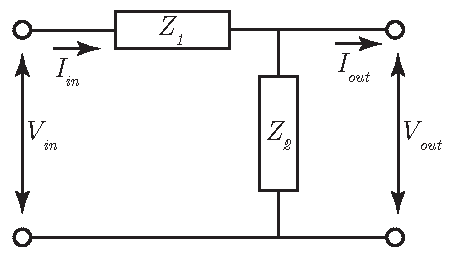
\includegraphics[width=3in]{twpa_theory/series_and_shunt_Z_network}
\end{center}
\caption[Generic series and shunt impedance network]{General two-port network under consideration, with one series impedance $Z_1$ and one shunt impedance $Z_2$.  Note current and voltage conventions.}
\label{fig:Znet}
\end{figure*}

We can easily derive the ABCD matrix for the general network shown in Fig. \ref{fig:Znet} using Kirchoff's laws.  This network is general enough to cover lots of interesting cases.  The voltage and current at the output are
\begin{equation}
V_{out} = V_{in} - I_{in} Z_1
\label{eq:volt}
\end{equation}
\begin{equation}
I_{out} = I_{in} - V_{out}/Z_2 = (-1/Z_2)V_{in} + (1 + Z_1/Z_2) I_{in}
\label{eq:curr}
\end{equation}
so the ABCD matrix of this network is
\begin{equation}
\left( \begin{array}{cc}
1 & -Z_1 \\
-1/Z_2 & 1+Z_1/Z_2 \end{array} \right).
\label{eq:2ZABCD}
\end{equation}
Thus, from (\ref{eq:disp}), for arbitrary series and shunt impedances the dispersion relation of this network is
\begin{equation}
ka = \cos^{-1}(1 + Z_1/2Z_2).
\label{eq:twoZdisp}
\end{equation}
For a simple LC ladder transmission line, $Z_1 = i \omega L$ and $Z_2 = 1/i \omega C$ so the dispersion relation is
\begin{equation}
ka = \cos^{-1}\left(1 - \frac{\omega^2}{(2 \omega_0)^2}\right),
\label{eq:LC_ladder_disp}
\end{equation}
where $\omega_0 = 1/\sqrt{LC}$.  A plot of this equation is shown as the red trace in Figure \ref{fig:JJ_ladder_disp}, in normalized units.  The characteristic frequency $\omega_0$ is called the \textit{plasma frequency} of the transmission line, corresponding to the resonance frequency of each rung of the LC ladder.  Above twice the plasma frequency, the dispersion relation is imaginary and there is no solution to the wave equation that permits a traveling mode, implying the existence of a very opaque stop-band above $2\omega_0$.  At frequencies much smaller than $\omega_0$, the dispersion relation is well-approximated as linear.

\begin{figure*}
\begin{center}
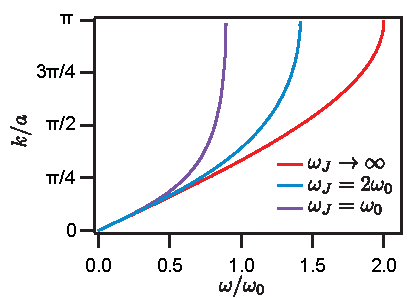
\includegraphics[width=2.75in]{twpa_theory/JJ_ladder_disp}
\end{center}
\caption[Dispersion relation for small-signal junction-loaded transmission line]{Dispersion relations for various ratios of plasma frequencies.  The case where the inductance has no parallel capacitance is plotted in red.  As the junction plasma frequency is reduced (finite shunt capacitance across the inductor), the cutoff frequency decreases and the curvature of the band increases.}
\label{fig:JJ_ladder_disp}
\end{figure*}

For the junction-loaded transmission line from Figure \ref{fig:TWPA_circuit_model}, the Josephson inductance is shunted by the intrinsic capacitance of the junction, so $Z_1$ is the parallel combination of $Z_L$ and $Z_{C_j}$.  This leads to a slightly more complex form
\begin{equation}
ka = \cos^{-1}\left(1 - \frac{\omega^2}{2 \omega_0^2 (1 - \omega^2/\omega_J^2)}\right)
\label{eq:JJ_ladder_disp}
\end{equation}
where we have introduced another characteristic frequency $\omega_J = 1/\sqrt{L C_J}$, the plasma frequency of the Josephson junction.  The net effect on the dispersion relation is to introduce an additional curvature into the band, and also modify the location of the edge of the stop band.  The cutoff frequency is now given by
\begin{equation}
\omega_C = \frac{2 \omega_0}{\sqrt{1 - 4 \omega_0^2/\omega_J^2}}.
\label{eq:JJ_disp_cutoff}
\end{equation}
In the small-signal regime, the phase matching condition $2 k_p = k_s + k_i$ will be satisfied for a perfectly linear dispersion.  The curvature of the band introduced by the two plasma frequencies serves to spoil this linearity for frequencies at an appreciable fraction of the cutoff frequency, and it is this band curvature that will be partially responsible for determining the amplification bandwidth of the JTWPA.

It is at this point that we must determine some method to create a local modification in the dispersion relation to satisfy (\ref{eq:deltak}).  There are many techniques known in nonlinear optical system to accomplish this \cite{armstrong_interactions_1962,Agrawal2012}; however, all of those systems are generally faced with the constraint of a very short optical wavelength, requiring schemes that work on the basis of distributed geometry.  Because the JTWPA is a microwave metamaterial and is already composed of deep-subwavelength elements, we can take a completely different and new approach to the problem.

\begin{figure*}
\begin{center}
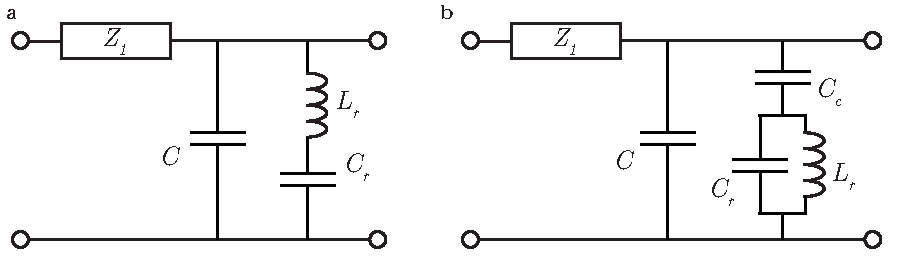
\includegraphics[width=6in]{twpa_theory/shunt_resonators}
\end{center}
\caption[Shunt resonator topologies]{Shunt resonator topologies: \textbf{a} series LC shunt; \textbf{b} capacitively-coupled parallel LC shunt.}
\label{fig:shuntres}
\end{figure*}

Because we seek a narrowband modification to the dispersion relation, we can start with the most common narrowband circuit topology: a resonator.  The most straightforward way to add a resonance is the addition of a series LC resonator in parallel with the capacitance to ground as shown in Figure \ref{fig:shuntres}a.  This configuration can be understood as a common circuit topology for implementing a notch filter.  Nearby but outside the stop-band of this filter the linear wave propagation will be slightly altered, leading to an increase in wavevector.  An alternative to the series LC shunt resonator is to add a capacitvely-coupled parallel LC resonator, shown in Figure \ref{fig:shuntres}b.  By introducing the coupling capacitor $C_c$, this topology has an extra degree of freedom compared to the series LC resonator, allowing the impedance of the resonator and the coupling to the transmission line to be adjusted independently.  This extra freedom will turn out to be crucial in fabricating a realistic device, so we will focus only on the parallel LC configuration.

To find the dispersion relation of these networks all we need to do is calculate $Z_1$ and $Z_2$ and plug it into (\ref{eq:twoZdisp}).  For the parallel LC shunt,
\begin{equation}
Z_1 = Z_L || Z_{C_j} = \left( \frac{1}{i \omega L} + i \omega C_j \right)^{-1}
\label{eq:Z1_parallel}
\end{equation}

\begin{equation}
Z_2 = Z_C || Z_{res}
\label{eq:Z2_parallel}
\end{equation}
where
\begin{equation}
Z_{res} = (Z_{C_c} + (Z_{C_r} || Z_{L_r})) = \frac{1 - \omega^2 L_r (C_r + C_c)}{i \omega C_c (1 - \omega^2 L_r C_r)}
\label{eq:Zres}
\end{equation}
Usually, identifying $L_r C_r = 1/\omega_r^2$ would simplify this expression, but the presence of the coupling capacitor effectively pulls the resonance frequency and makes this substitution somewhat less helpful.  Expanding (\ref{eq:twoZdisp}) delivers the dispersion relation for the junction-loaded, capactively-coupled-parallel-LC-resonator-shunted (whew) transmission line:
\begin{equation}
ka = \cos^{-1}\left( 1 - \frac{\omega^2 L (C ( 1 - \omega^2 L_r (C_r + C_c) ) + C_c (1 - \omega^2 L_r C_r) ) }{2(1 - \omega^2 / \omega_J^2)(1 - \omega^2 L_r (C_r + C_c))} \right)
\label{eq:fulldisp}
\end{equation}

\begin{figure*}
\begin{center}
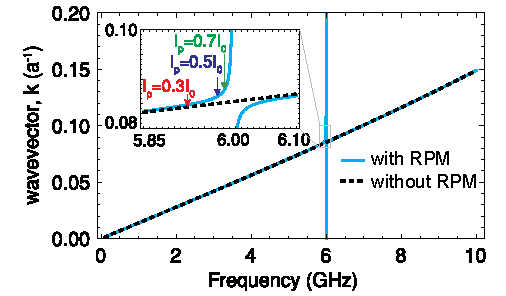
\includegraphics[width = 3.38in]{twpa_theory/disp_rpm}
\end{center}
\caption[JTWPA dispersion relation with and without RPM]{Plot of the exact JTWPA dispersion relation for $C_j$=329 fF, $L$=100 pH, $C$=39 fF, $C_c$=10 fF, $C_r$=7.036 pF, $L_r$=100 pH, and $I_0$=3.29 $\mathrm{\mu A}$.  The dispersion relation without RPM loading resonators is plotted as a dashed line and is approximately linear, though a slight curvature can be seen above 8 GHz.  The effect of the RPM loading resonators is plotted in cyan; in a very narrow band around the resonance frequency at 6 GHz, the dispersion relation diverges.  This is more clearly seen in the inset plot.  The colored labels and arrows indicate the pump frequency at which the power-dependent phase shift (proportional to $\kappa \propto (I_p/I_0)^2$) is perfectly compensated, enabling perfect phase matching.  Adapted from reference \cite{OBrien2014}.}
\label{fig:disp_rpm}
\end{figure*}

We can make the small-angle approximation in $ka$ to reduce the complexity of the problem somewhat.  This is a reasonable approximation to provide a more intuitive expression, as we expect to need a very small fractional shift in the wavevector to compensate the power-dependent phase shift.  We approximate the dispersion relation to second order in $ka$ as $2 \cos(ka) \approx 2 - (ka)^2$.  Additionally, we can assume that the junction plasma frequency $\omega_J$ is large compared to $\omega$.  This eliminates the first term in the denominator of (\ref{eq:fulldisp}).  Rearranging some terms, this gives a form in which it is easier to identify the effect of the resonator:
\begin{equation}
(ka)^2 \approx \frac{\omega^2}{\omega_0^2} + \frac{\omega^2 L C_c (1 - \omega^2 L_r C_r)}{1 - \omega^2 L_r (C_r + C_c)}
\label{eq:approxdisp}
\end{equation}
The first term is the linear dispersion of the unloaded transmission line, while the second term is the loading effect of the resonator.  We identify the loaded frequency of the resonator as the center frequency of the dispersion feature at $\omega_r = 1 / \sqrt{L_r (C_r + C_c)}$ where the denominator in the second term goes to zero.  Note that for frequencies slightly below $\omega_r$, the second term is positive, and we have achieved the desired local shift in the wavevector needed to achieve phase matching.  We have named this new phase matching technique ``resonant phase matching'' (RPM).  A plot of the resulting dispersion relation is shown in Figure \ref{fig:disp_rpm}, demonstrating the creation of the stop band and showing the divergence of the dispersion relation near $\omega_r$.



\section{Amplifier performance with resonant phase matching}\label{s:rpm_perf}

\subsection{Gain and bandwidth}

\begin{figure}
\begin{center}
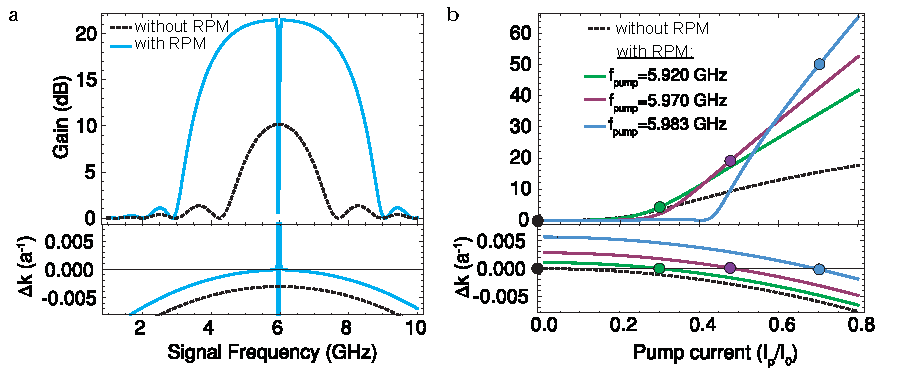
\includegraphics[width = 6in]{twpa_theory/twpa_gain}
\end{center}
\caption[JTWPA gain and phase mismatch]{Gain of a 2000 unit cell JTWPA with and without RPM loading structures. \textbf{a} The gain as a function of signal frequency in dB with RPM (cyan) and without (black dashed) for a pump current of 0.5$I_0$ and a pump frequency of 5.97 GHz.  The plot below shows the phase mismatch with RPM (cyan) and without (black dashed).  The device with RPM is perfectly phase matched at zero detuning, and becomes poorly phase matched due to the curvature of the dispersion relation as the detuning is increased.  \textbf{b} The peak gain as a function of pump current without RPM (black dashed) and with RPM for three different pump frequencies, which phase match the parametric amplification process for pump currents of 0.3 $I_0$ (green), 0.5 $I_0$ (purple), and 0.7 $I_0$ (cyan). The plot below shows the phase mismatch as a function of pump current. The dots mark the pump current where perfect phase matching is achieved.  Adapted from reference \cite{OBrien2014}.}
\label{fig:twpa_gain}
\end{figure}

Now that we have created a dispersion relation that exactly satisfies (\ref{eq:deltak}), we expect to achieve gain which grows exponentially in the length of the device.  To understand the frequency dependence of the gain, we need to examine the exact form of the exponential gain coefficient (\ref{eq:g}).  From Appendix \ref{a:twpa_paramp}, the frequency and wavevector dependence of the coupling coefficients $\kappa_s$ and $\kappa_i$ are
\begin{align}
\kappa_s &\propto \frac{(2 k_p - k_i) k_s k_i}{\omega_s^2} \\
\kappa_i &\propto \frac{(2 k_p - k_s) k_s k_i}{\omega_i^2}.
\end{align}
Re-expressing $\omega_s = \omega_p + \Delta$, $\omega_i = \omega_p - \Delta$, and assuming for the moment an approximately linear dispersion relation $k \propto \omega$, we can write the frequency dependence of $g$ for $\Delta k = 0$ as
\begin{equation}
g \propto \sqrt{\omega_p^2 - \Delta^2}.
\label{eq:g_vs_f}
\end{equation}
Thus, even for perfect phase matching, we expect the gain to decrease as the pump-signal detuning increases.  Due to the finite curvature of the dispersion relation, the phase matching will also only be close to perfect at small detuning, so this will also contribute to setting the bandwidth of the amplifier.

In Figure \ref{fig:twpa_gain}a, we show the gain and phase mismatch for a 2000 unit cell device with pump current $I_p = 0.5 I_0$ at $f_p = 5.97$ GHz and the same device parameters listed in Figure \ref{fig:disp_rpm}.  For perfect phase matching, we predict a gain of just over 20 dB with a very large bandwidth, nearly an entire octave centered at 6 GHz.  Without the phase matching improvement from RPM, the gain is only 10 dB with a bandwidth of a bit under 2 GHz.  The bandwidth is set by a combination of the phase mismatch due to the band curvature and the detuning dependence (\ref{eq:g_vs_f}).  The effect of RPM can be understood well by the bottom plot in \ref{fig:twpa_gain}b; for low pump powers, the phase mismatch is positive, and decreases to cross zero.  In the vicinity of the zero crossing, the four-wave mixing process is efficient and the gain increases exponentially in the pump current.

\begin{figure}
\begin{center}
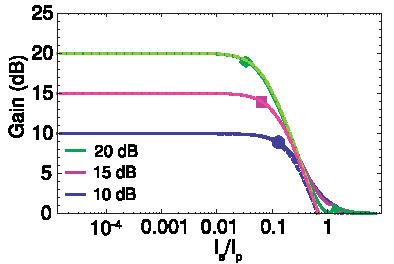
\includegraphics[width = 2.63in]{twpa_theory/twpa_comp}
\end{center}
\caption[JTWPA gain compression]{Amplifier gain as a function of input signal current, normalized to the pump current, for a small signal gain of 10, 15, and 20 dB obtained with a pump current of $0.5 I_0$ and device lengths of 1150, 1530, and 1900 unit cells. The approximation for the gain depletion (dashed lines) from (\ref{eq:gen_comp}) is in excellent agreement with the result obtained by solving the full nonlinear dynamics (solid lines).   Adapted from reference \cite{OBrien2014}.}
\label{fig:twpa_comp}
\end{figure}

\subsection{Dynamic range}

The upper limit of the dynamic range of a parametric amplifier is given by pump depletion: the pump transfers energy to the signal and idler which reduces the parametric gain. To investigate this regime, we solve for the coupled wave equations without the undepleted pump approximation. This derivation appears as Appendix 4 in reference \cite{OBrien2014}, and the resulting curves are plotted as solid lines in Figure \ref{fig:twpa_comp}. The gain as a function of input signal power calculated from the full analytical expression is in excellent agreement with the approximate, general solution for pump depletion in a four-wave parametric amplifier \cite{kylemark_semi-analytic_2006}:
\begin{equation}
G=\frac{G_0}{1+2 G_0 I_{s}^2/I_{p}^2} \label{eq:gen_comp}
\end{equation}
where $G_0$ is the small signal power gain in linear units and $I_{s}$ and $I_{p}$ are the input signal and pump currents. From (\ref{eq:gen_comp}), the gain compression point is approximately $P_{1 \rm dB}=P_{p}/(2 G_0)$. Thus, the threshold for gain saturation is independent of the specific device configuration and depends only on the small signal gain and the pump power. For the device parameters listed previously, the gain as a function of input signal current is plotted for three values of the small signal gain in Figure \ref{fig:twpa_comp}. The signal current at which the gain drops by 1 dB is marked. For a pump current of $0.5 I_0$, the signal power where the gain decreases by 1 dB is $-87$, $-93$, and $-98$ dBm for a small signal gain of 10, 15, and 20 dB, respectively. These gain compression points are consistent with the approximate relation with the pump power of -69 dBm.  A 1 dB input compression power of -98 dB is about 12 dB higher than achieved by any JPA with comparable gain.

\subsection{Parameter regime}\label{s:twpa_param}

The parameters chosen for these theory plots are the result of extensive engineering using the full theory of the device.  Simplifying the expression for the gain by assuming perfect phase matching and neglecting the effects of the resonant element and the junction resonance on the dispersion, we find that the exponential gain coefficient is directly proportional to the wave vector $g\propto k_p I_p^2/I_0^2$. Thus, for a fixed pump strength relative to the junction critical current, the gain coefficient is proportional to the electrical length. In other words, a larger wave vector and thus a slower effective wave propagation velocity leads to a larger effective nonlinearity due to the higher energy density; this effect is well known in photonic crystals \cite{soljacic_photonic-crystal_2002}. Because the characteristic impedance is designed to be $Z \approx \sqrt{L/(C+C_c)} \approx 50$ $\Omega$, the ratio of the inductance and capacitance is fixed. The wave vector is proportional to the product of the capacitance and inductance $k \approx (\omega/a) \sqrt{L(C+C_c)}$.

Increasing both the capacitance and inductance or decreasing the unit cell size are effective strategies for increasing the gain per unit length while maintaining impedance matching for 50 $\Omega$ feedlines.  However, because the junction critical current $I_0$ (and the resulting maximum pump power) scales inversely with the inductance \eqref{eq:LJ}, increasing the wavevector to increase the gain also decreases the dynamic range of the amplifier.  Additionally, the minimum size of the unit cell is constrained due to the finite physical extent of the capacitors and inductors. The parameters in the design discussed here sit in a surprisingly small area of the total parameter space where we realize an amplifier that simultaneously achieves large gain, large bandwidth, and large dynamic range.

Although the very large gain operation shown in the top panel of \ref{fig:twpa_gain}b is impressive at first glance, operation with such large gain is unrealistic due to several physical constraints.  First, the total power in a pump wave with $I_p = I_0 \sim 5$ $\mu$A is $P_p \sim -62$ dBm.  Enforcing our general constraint on power scales for linear operation of a parametric amplifier from section \ref{s:jpa_perf} and formalized in (\ref{eq:gen_comp}), our amplified output signal power should be no larger than $P_p - 20$ dB.  Without any signal at the input, the amplifier must still amplify any input noise present, which corresponds to at least $\hbar \omega$ per mode of quantum fluctuations across the entire bandwidth of the device \eqref{eq:half_quantum}.  This results in an input noise power roughly given by $P_Q \approx \hbar \omega B = -108$ dBm for $B = 4$ GHz centered at $\omega/2 \pi = 6$ GHz.  In order to satisfy $P_Q + G < P_p - 20$ dB, the gain must be no larger than about 26 dB for the input noise power to not drive the amplifier into gain compression.  This constraint could be relaxed by reducing the bandwidth, but gain exceeding 20 dB is not normally necessary to achieve quantum-limited operation for the whole measurement system.

A further constraint comes from the fact that we have so far ignored the possible effect of multiple reflections at the input and output of the amplifier.  In any real device, the matching between the nonlinear transmission line and the linear input and output feedlines will be imperfect, so some fraction of the amplified signal will be reflected from the output back to the input.  If the reflection coefficient is $R$ in dB, then a signal at the input amplified by the gain $G$ reflects back from the output at the level of $G+R$ and is reflected at the input back into the amplifier again at $G+2R$.  For the amplifier to be stable, this feedback gain must be less than 0 dB; realistically, we would like it to be much smaller than 0, otherwise we will set up a large standing wave inside the amplifier which will produce large ripples in the gain profile at harmonics of twice the frequency corresponding to the electrical length of the JTWPA.  For typical microwave devices, $R = -20$ dB is considered to be well-matched, and reducing this further is quite challenging especially in a broadband circuit.  Thus, if $G$ is larger than 40 dB, the amplifier will be unstable; moreover, if we want the total reflection $G+2R$ to be -20 dB or better, $G \lesssim 20$ dB.

\subsection{Effect of finite losses}\label{s:twpa_loss_theory}

Although superconducting circuits are generally low-loss, there will still be some attenuation at microwave frequencies due to effects such as dielectric loss.  To describe the attenuation of propagating waves in the transmission line, we use a complex wavevector, $k=k'+i k''$, where the real ($k'$) and imaginary ($k''$) components describe phase evolution and attenuation, respectively, as a function of position. Including material damping, the differential equation for the signal and idler amplitudes in a rotating frame is $\mathbf{u}'(x)=\mathbf{M}(x) \mathbf{u}(x)$ where $\mathbf{u}=[a_s  ~ a_i]^T$ and 
\begin{align}
\mathbf{M}_f = 
\begin{bmatrix}
- i\frac{\Delta k}{2}-k''_s & i\kappa_s \\
-i\kappa^*_i            & i\frac{\Delta k}{2}-k''_i
\end{bmatrix} \label{eq:signallossy}
\end{align} 
where $\Delta k=2k_p-k_i-k_s+2\alpha_p-\alpha_s-\alpha_i$ is the phase mismatch, $k_{p,s,i}$ are the wavevectors in the weak field limit, $\kappa_{s,i}$ are the coupling constants for the signal and idler, $\alpha_{p,s,i}$ describe the nonlinear phase shifts (defined in Appendix \ref{a:twpa_paramp}), and $k''_{s,i}$ are the imaginary components of the signal and idler wavevectors. In a lossy nonlinear transmission line, the pump amplitude decays with position leading to position dependent phase mismatch and coupling constants; however, if the attenuation is small, the effect of pump attenuation can be approximated by a position independent phase mismatch and coupling constant with a reduced pump amplitude $A'_p=A_p\exp({-k''_p L/2})$. The solution to these coupled differential equations is then $\mathbf{u}(x)=e^{\mathbf{M}x} \mathbf{u}(0)$. The signal amplitude in the lab frame is $a_s(x)=[1,0]\mathbf{u}(x)[1,0]^T e^{i(\Delta k/2 + \alpha_s)x}$ with gain $G=|a_s(L)/a_s(0)|^2$. 

\subsection{Quantum efficiency with distributed loss}\label{s:twpa_dist_loss}

Because the loss in the JTWPA is distributed along the amplifier, losses further down the device should participate less strongly in setting the quantum efficiency than losses near the beginning.  This follows from the same intuition that losses following a high-gain amplifier should not participate strongly in setting the noise temperature of the system as long as the gain is significantly larger than the loss.  To account for the reduction in quantum efficiency attributable to distributed loss in the amplifier, we model the JTWPA as a series of cascaded ideal phase-preserving amplifiers and lumped attenuation elements, shown schematically in Fig. \ref{fig:chained_caves_amp}.

\begin{figure*}
\begin{center}
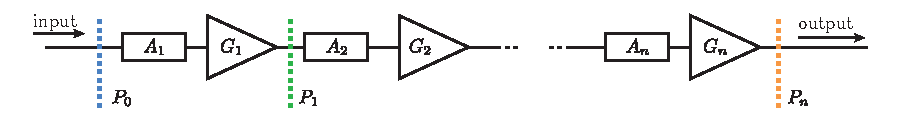
\includegraphics[width=6in]{twpa_theory/chained_caves_amp}
\end{center}
\caption[Distributed amplifier loss model]{Block diagram of the model for distributed loss and gain, showing a series of discrete attenuators $A_i$ each followed by a ideal phase-preserving amplifier with gain $G_i$.}
\label{fig:chained_caves_amp}
\end{figure*}

At the input to the amplifier at plane $P_0$ (blue dashed line) we have input noise $N_0 = N_Q = 1/2$, in units of quanta.  To calculate the noise at plane $P_1$ (green dashed line) following the lumped attenuation $A_1$ and gain element $G_1$ (both given in linear power units), we must take into account the additional quantum fluctuations added by the attenuation, $N_{\textrm{atten}} = N_Q(1-A_1)$, and the ideal phase-preserving amplifier
\begin{equation}
N_{\textrm{amp}} = N_Q(1-1/G_1)
\label{eq:caves_noise}
\end{equation}
(referred to the amplifier's input) \cite{Caves1982a}.  The total noise at plane $P_1$ is thus $N_1 = G_1 ( N_0 A_1 + N_Q (1 - A_1) + N_Q(1 - 1/G_1))$ \footnote{Our choice of ordering of the attenuation element and the gain element is arbitrary, though placing the attenuation block first gives a lower bound on $\eta$ rather than an upper bound.  For many hundreds of elements, the noise calculated for both orderings converge.}.  We can generalize this into a recurrence relation
\begin{equation}
N_i = N_{i-1}A_i G_i + N_Q (1 - A_i) G_i + N_Q (G_i - 1)
\label{eq:caves_recurr}
\end{equation}
which can be summed numerically for any distribution of $A_i$ and $G_i$ to find the total noise at the output $N_n$.  Referring the noise back to the input of the amplifier by dividing by the total transmission $T = \prod_{i=1}^n A_i G_i$ allows the expected quantum efficiency to be calculated as
\begin{equation}
\eta = (N_n / T)^{-1}
\label{eq:eta_D}
\end{equation}
assuming that the total amplifier gain is large enough to saturate (\ref{eq:caves_noise}) in the absence of loss.







